\documentclass[
  a4paper,               % A4-Papier
  twoside,               % zweiseitig
  DIV=12,                % Zwölfteilung der Seite
  BCOR=8mm,              % 8mm Korrektur für Bindung
  headinclude=true,      % Header hinzufügen
  footinclude=false,     % Footer nicht hinzufügen
  numbers=noenddot,      % keine Punkte nach Kapitelnummern
  headheight=40pt,       % Höhe des Header-Blocks
  11pt]{scrartcl}        % Schriftgröße

\usepackage[T1]{fontenc}
\usepackage[utf8]{luainputenc}
% not in use. use XeLaTeX compiler and fontspec if necessary.
%\usepackage[math-style=TeX, bold-style=TeX]{unicode-math}
\usepackage[ngerman]{babel}
\usepackage{amsfonts, amsmath, amsthm}
\usepackage{graphicx}
\usepackage{textcomp}
\usepackage{gensymb}
\usepackage{hyperref}
\usepackage{wrapfig}
\usepackage{xcolor}
\usepackage{todo}
\usepackage{booktabs}
\usepackage{pdfpages}
\xdefinecolor{unifarbe}{RGB}{0,75,90}

\usepackage{sectsty}
\chapterfont{\color{unifarbe}}  % sets colour of chapters
\sectionfont{\color{unifarbe}}  % sets colour of sections
\subsectionfont{\color{unifarbe}}  % sets colour of subsections
\begin{document}

\begin{titlepage}

\flushleft
\includegraphics[width=0.5\textwidth]{./Logo_Uni_Luebeck_CMYK} \\[1cm]
\color{unifarbe}
\begin{center}
\textbf{\Huge Bachelorprojekt} \\[0.5cm]
\textbf{\Huge Optimierung biologisch-realistischer Neuronenmodelle}\\[0.5cm]

Institut für Robotik und Kognitive Systeme\\[2.5cm]
\textbf{\Large Dokumentation}\\[1.5cm]

Szymon Bereziak\\
Moritz Dannehl\\
Chris Girth\\
Can Kalelioglu\\
Julian Wolff\\
\end{center}

\vfill
\today

\end{titlepage}
\tableofcontents\newpage
\section{Einführung}
\subsection{Ziel des Projektes}

Mithilfe von künstlichen neuronalen Netzen wird versucht, Strukturen des menschlichen Gehirns zu simulieren. Die verwendeten Simulationen basieren dabei auf sehr vielen Parametern, deren Optimierung eine sehr langwierige Aufgabe darstellt. Es wurde im Rahmen dieses Projektes ein Framework erstellt, welches als Schnittstelle zwischen solchen Simulationen und Optimierungsalgorithmen fungiert. Dabei waren vor allem eine Modularisierung zwecks Erweiterbarkeit sowie eine einfache Bedienbarkeit über eine grafische Oberfläche Zentrum der Entwicklung.
\section{Features}
\begin{itemize}
\item einfache Anbindung eines (neuen) Frontends möglich durch ein simples Nachrichtenprotokoll
\item einfaches Hinzufügen von neuen Algorithmen
\item Modularisierung erlaubt komplettes Austauschen einzelner Module ohne die Kernlogik zu kennen
\item verteiltes Arbeiten möglich durch Anbindung des Simulationsclusters über SSH oder andere Protokolle
\item Multithreading bereits nativ in Kernlogik implementiert; Kern verwaltet verschiedene Läufe von Algorithmen selbstständig
\item kein aktives Warten notwendig; bei Terminierung eines Algorithmus' wird das Frontend automatisch benachrichtigt

\end{itemize}


\section{Architektur}
Das Framework ist in zwei Teile gegliedert. Der \emph{Kern} verwaltet selbstständig alle Algorithmen und spricht die Simulation an. Die Kommunikation zwischen dem Kern und der \emph{Benutzerschnittstelle} erfolgt über eine nachrichtenbasierte \emph{Kommunikationsschnittstelle}. Die Benutzerschnittstelle kann eine grafische Benutzeroberfläche oder ein Kommandozeileninterface sein. Über die Kommunikationsschnittstelle werden dem Kern Befehle erteilt, die das Einladen von Konfigurationen, Setzen von Parametern, Starten und Stoppen von Algorithmen sowie Statusabfragen umfassen.
\subsection{Kern}
grumpf
\subsection{GUI}
% vim:ft=tex
\begin{samepage}
Die GUI besteht aus den folgenden Komponenten: \\
\textbf{mainframe}. Dient dem Starten, Stoppen, Überwachen und Speichern der Berechnungen.\\
\textbf{addframe}. Ermöglicht die Auswahl der Optimierungsalgorithmen und das Setzen der Startparameter.\\
\textbf{sshframe}. Oberfläche zur Eingabe der SSH-Daten.
\end{samepage}

\section{Benutzerhandbuch}
\subsection{Ausführen der Anwendung}
Zur Ausführung sind die Pakete \texttt{python3} und \texttt{sshpass} notwendig.\\
Die Anwendung kann als Kommandozeilenanwendung mithilfe des Befehls \texttt{python3 main.py} oder alternativ mit grafischer Oberfläche mithilfe des Befehls \texttt{python3 main.py -{}-gui} ausgeführt werden.
\subsection{CLI}
Wird die Anwendung als Kommandozeilenanwendung gestartet, so kann sie mittels der folgenden Befehle gesteuert werden:\\
\begin{tabular}{p{0.4\linewidth}|p{0.55\linewidth}}
	\toprule
	Befehl & Auswirkung\tabularnewline
	\midrule
	\texttt{help} & Liefert eine Liste möglicher Befehle, ähnlich dieser
	Tabelle\tabularnewline
	\texttt{get\ algorithms} & liefert eine Liste von implementierten
		Algorithmen\tabularnewline
	\texttt{get\ algorithms\ \textless{}name\textgreater{}} & liefert die
	möglichen Parameter für den angegebenen Algorithmus\tabularnewline
	\texttt{get\ config} & liefert alle in der Konfigurationsdatei
	vorhandenen Sektionen\tabularnewline
	\texttt{get\ config\ \textless{}sec\textgreater{}} & liefert alle
	Optionen unter der gegebenen Sektion\tabularnewline
	\texttt{get\ config\ \textless{}sec\textgreater{}\ \textless{}opt\textgreater{}}
	& liefert den Wert der angegebenen Option\tabularnewline
	\texttt{set\ config\ \textless{}sec\textgreater{}\ \textless{}opt\textgreater{}\ \textless{}val\textgreater{}}
	& Setzt die angegebene Option auf den angegebenen Wert\tabularnewline
	\texttt{set\ password} & Öffnet eine Passworteingabe zur Eingabe des
	Passworts der SSH-Verbindung zum neuronalen Netz\tabularnewline
	\texttt{save\ config} & Speichert die Änderungen in der
	Konfigurationsdatei\tabularnewline
	\texttt{start\ \textless{}algorithm\textgreater{}\ \textless{}params...\textgreater{}}
	& Startet einen Optimierungsalgorithmus mit den gegebenen
	Parametern\tabularnewline
	\bottomrule
\end{tabular}\\
\newline\\
Bevor eine Optimierung gestartet wird sollten folgende Befehle
aufgerufen werden:\\
\begin{tabular}{p{0.4\linewidth}|p{0.55\linewidth}}
	\toprule
	Befehl & Auswirkung\tabularnewline
	\midrule
	\texttt{set\ password} & Setzt das SSH Passwort\tabularnewline
	\texttt{set\ config\ SSH\ host\ \textless{}user@ip\textgreater{}} & Setzt
	die Serveradresse\tabularnewline
	\texttt{set\ config\ SSH\ net\ \textless{}cmd\textgreater{}} & Setzt
	den Befehl zur Ausführung des neuronalen Netzes\tabularnewline
	\texttt{set\ config\ SSH\ analysis\ \textless{}cmd\textgreater{}} &
	Setzt den Befehl zur Ausführung der Analyse\tabularnewline
	\bottomrule
\end{tabular}\\
\newline\\
Anschließend können beliebige Optimierungsalgorithmen gestartet werden.\\
\newline\\
\begin{samepage}
Beispiel:\\
\texttt{
\noindent\hspace*{10mm}	>set config SSH host "bachelor1@localhost"\\
\noindent\hspace*{10mm}	>set config SSH net "cd  \raisebox{-0.6ex}{\~{ }}/acnet2 \&\& genesis acnet2.g"\\
\noindent\hspace*{10mm}	>set config SSH analysis "cd  \raisebox{-0.6ex}{\~{ }}/acnet2 \&\& python ./analysis.py"\\
\noindent\hspace*{10mm}	>save config\\
\noindent\hspace*{10mm}	>set password\\
\noindent\hspace*{10mm}	>start random\_search 4
	}\\
\end{samepage}
\subsection{GUI}
Wird das Programm mittels des Befehls
\begin{center}
\texttt{python3 main.py -{}-gui}
\end{center}
gestartet, öffnet sich das Hauptfenster der grafischen Benutzeroberfläche.
Abbildung 1 zeigt schematisch die Möglichkeiten, welche die GUI bietet:\\
\begin{figure}[h]
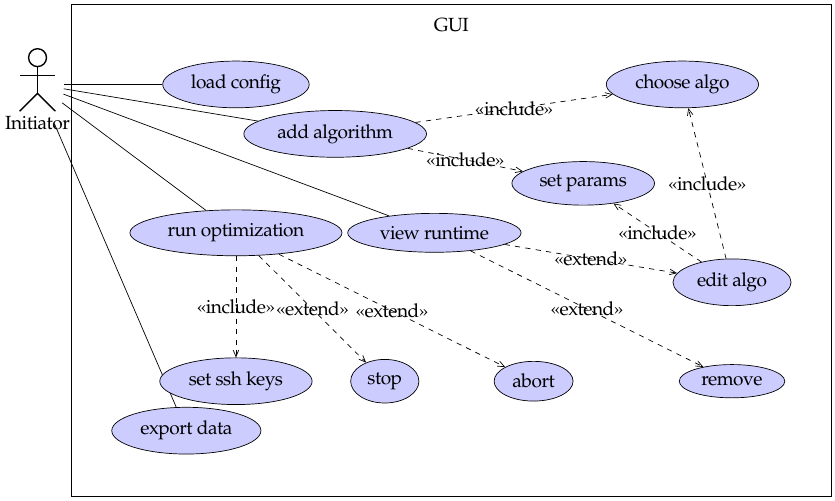
\includegraphics[scale = 2.5]{../presentation/GUI-use-case.png}
\caption{Use-case Diagramm GUI}
\end{figure}
\newpage
\begin{samepage}
Die folgende Tabelle liefert eine kurze Beschreibung der Funktionen:\\[0.5cm]
\begin{tabular}{p{0.4\linewidth}|p{0.55\linewidth}}
	\toprule
	Bezeichner & Funktion\tabularnewline
	\midrule
	\texttt{load session} & stellt die Daten einer zuvor gespeicherten Sitzung wieder her.\tabularnewline
	\texttt{add\ algorithm} & öffnet das addframe\tabularnewline
	\texttt{choose\ algorithm} & zeigt eine Auswahl der möglichen Algorithmen, von denen eine zu wählen ist.\tabularnewline
	\texttt{set\ params} & ermöglicht die Einstellung algorithmenspezifischer Parameter.\tabularnewline
	\texttt{view\ runtime} & liefert einen Überblick über die momentan gewählten Algorithmen und deren gegenwärtigen Status\tabularnewline
	\texttt{remove} & entfernt den ausgewählten Algorithmus\tabularnewline
	\texttt{run} & startet die Berechnung\tabularnewline
	\texttt{set\ ssh\ Keys} & Öffnet das Eingabefenster zur Eingabe des
	Passworts und anderer benötigter Parameter der SSH-Verbindung\tabularnewline
	\texttt{stop} & stoppt die Berechnung\tabularnewline
	\texttt{abort} & verwirft die Berechnung\tabularnewline
	\texttt{export data} & speichert die aktuelle Sitzung\tabularnewline
	\bottomrule
\end{tabular}\\
\end{samepage}

\end{document}
